%%%%%%%%%%%%%%% Pacotes utilizados
\documentclass[a4paper, 12pt]{article}
\usepackage[T1]{fontenc}
\usepackage[brazil]{babel}
\usepackage[utf8]{inputenc}
\usepackage{verbatim}
\usepackage[normalem]{ulem} %para 
\usepackage{indentfirst}
\usepackage{setspace}
\usepackage{float}
\usepackage{fancyhdr}
\usepackage{graphicx}


%%%%%%%%%%%%%%% Configurações
\setlength{\textwidth}{16cm}
\setlength{\textheight}{23cm}
\setlength{\evensidemargin}{-1cm} 
\setlength{\oddsidemargin}{0.5cm}
\setlength{\topmargin}{0cm}
\pagestyle{fancy}
\fancyhf{}
\lhead{\textbf{Nome:} Jhonatan Guilherme de Oliveira Cunha}
\rhead{\textbf{RA:} 2135590}
\cfoot{\thepage}
\hoffset= -0.4cm
\voffset=-0.9cm


%%%%%%%%%%%%% Início do documento
\begin{document}
	
	\hspace{5cm}
	
	\begin{large}
		\begin{center}
			\textbf{UNIVERSIDADE TECNOLÓGICA FEDERAL DO PARANÁ}\newline
			\textbf{CAMPUS CAMPO MOURÃO}
		\end{center}
	\end{large}
	
	\vspace{0.5cm}
	
	\begin{center}
		\textbf{BANDO DE DADOS 1 - LISTA TURMA 2020 MODELO ENTIDADE RELACIONAMENTO}
	\end{center}

	\vspace{0.5cm}
	

	
	
	\onehalfspacing
	\begin{enumerate}
		\item \textbf{[Empresa de TV]} Construa um modelo de entidade-relacionamento (MER) para uma empresa de TV que deseja desenvolver um banco de dados para armazenar dados sobre as séries que ela produz. Os dados incluem informações sobre os atores que participam da série e diretores que dirigem os episódios da série. Atores e diretores são empregados pela empresa. Uma série é dividida em episódios. Cada episódio pode ser transmitido em várias ocasiões. Um ator é contratado para participar de uma série, mas pode participar de muitas séries. Cada episódio de uma série é dirigido por um dos diretores, mas diferentes episódios podem ser dirigidos por diferentes diretores. Encontre atributos dos conjuntos de entidades e determine quais dos atributos que podem ser usados como chaves primárias.
		
		\begin{figure}[H]
			\centering
			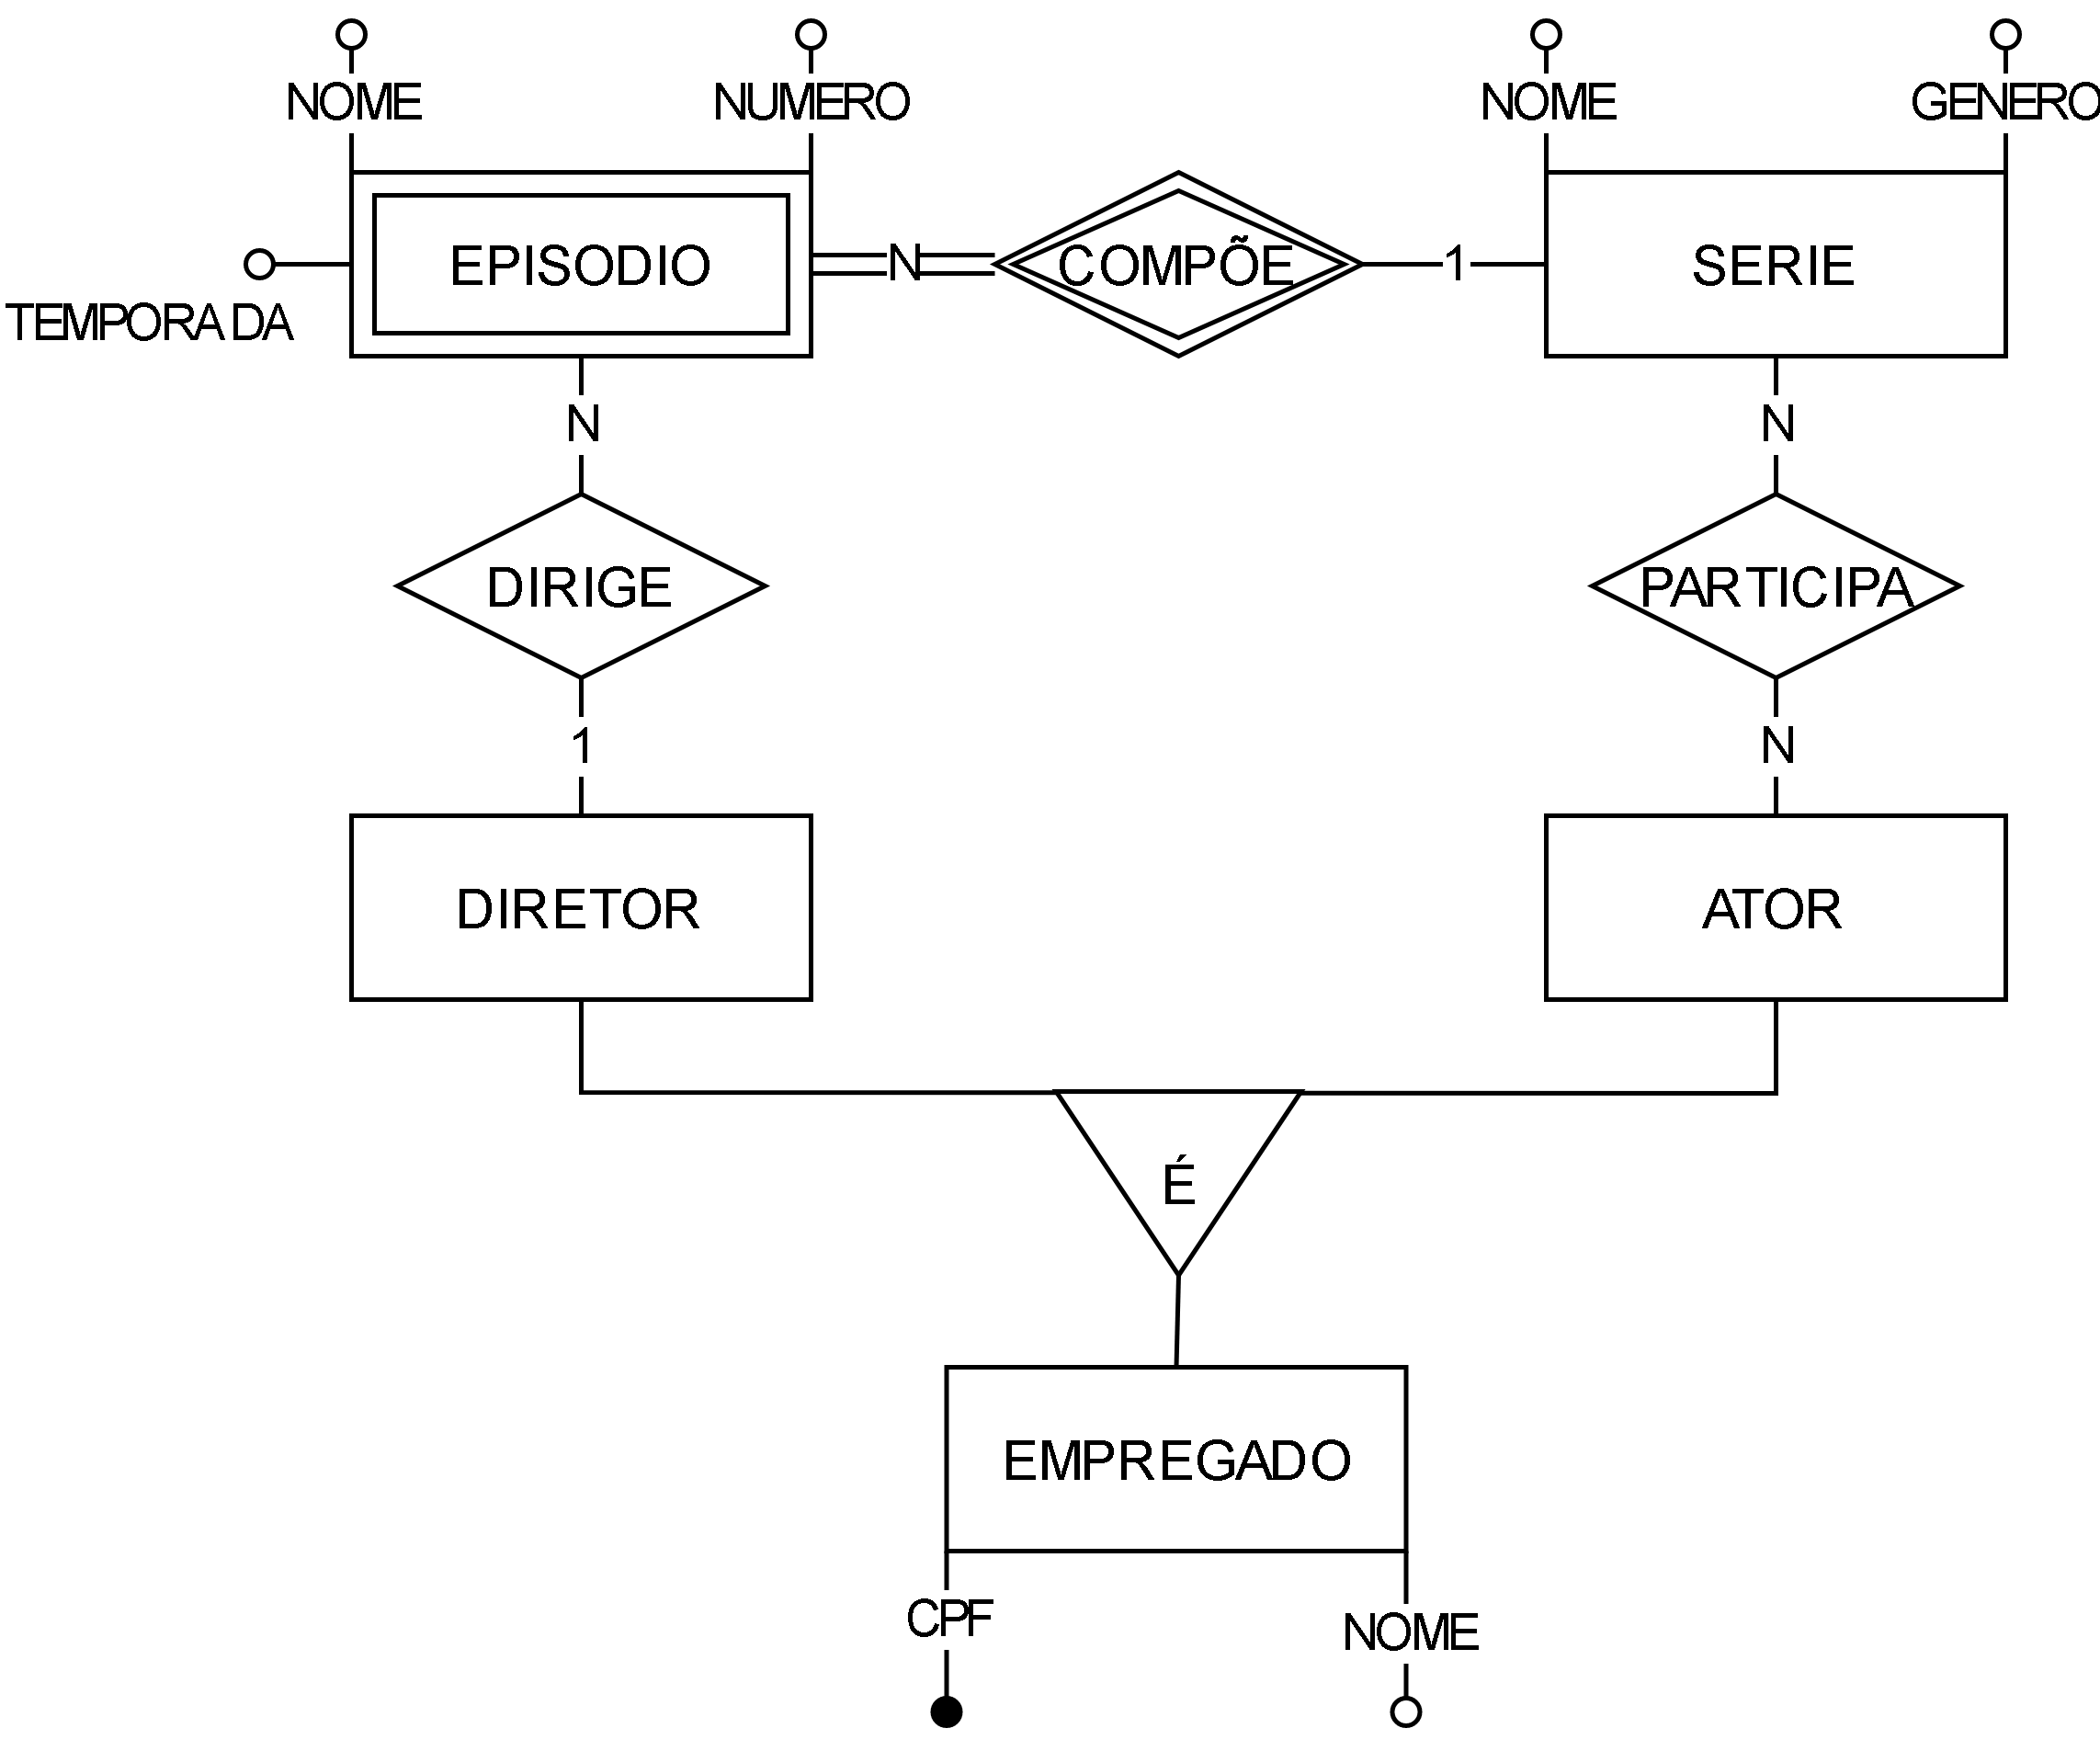
\includegraphics[width=0.85\textwidth]{empresaTV.png}
		\end{figure}
		
		
		\item \textbf{[Academia de Ginástica]} Construa um modelo de entidade-relacionamento (\textbf{MER}) para uma academia de ginástica que deseja construir uma base de dados para manter um controle do seu funcionamento. Os alunos são organizados em turmas associadas a um tipo específico de atividade (por exemplo, turma "Dança de Salão" da segunda-feira às 14h). As informações sobre uma turma são: identificador único, número de alunos, dia da semana, horário da aula, duração da aula, data inicial, data final e tipo de atividade. Cada turma é orientada por um único instrutor para o qual são cadastrados RG, nome, data de nascimento, titulação e todos os telefones possíveis para sua localização. Um instrutor pode orientar várias turmas que podem ser de diferentes atividades. Para cada turma existe um aluno monitor que auxilia o instrutor da turma, sendo que um aluno pode ser monitor no máximo em uma turma. Os dados cadastrados dos alunos são: código de matricula , data de matrícula, nome, endereço, telefone, data de nascimento, altura e peso. Um aluno pode estar matriculado em várias turmas se deseja realizar atividades diferentes e para cada matrícula é mantido um registro das ausências do aluno.
		
		\begin{figure}[H]
			\centering
			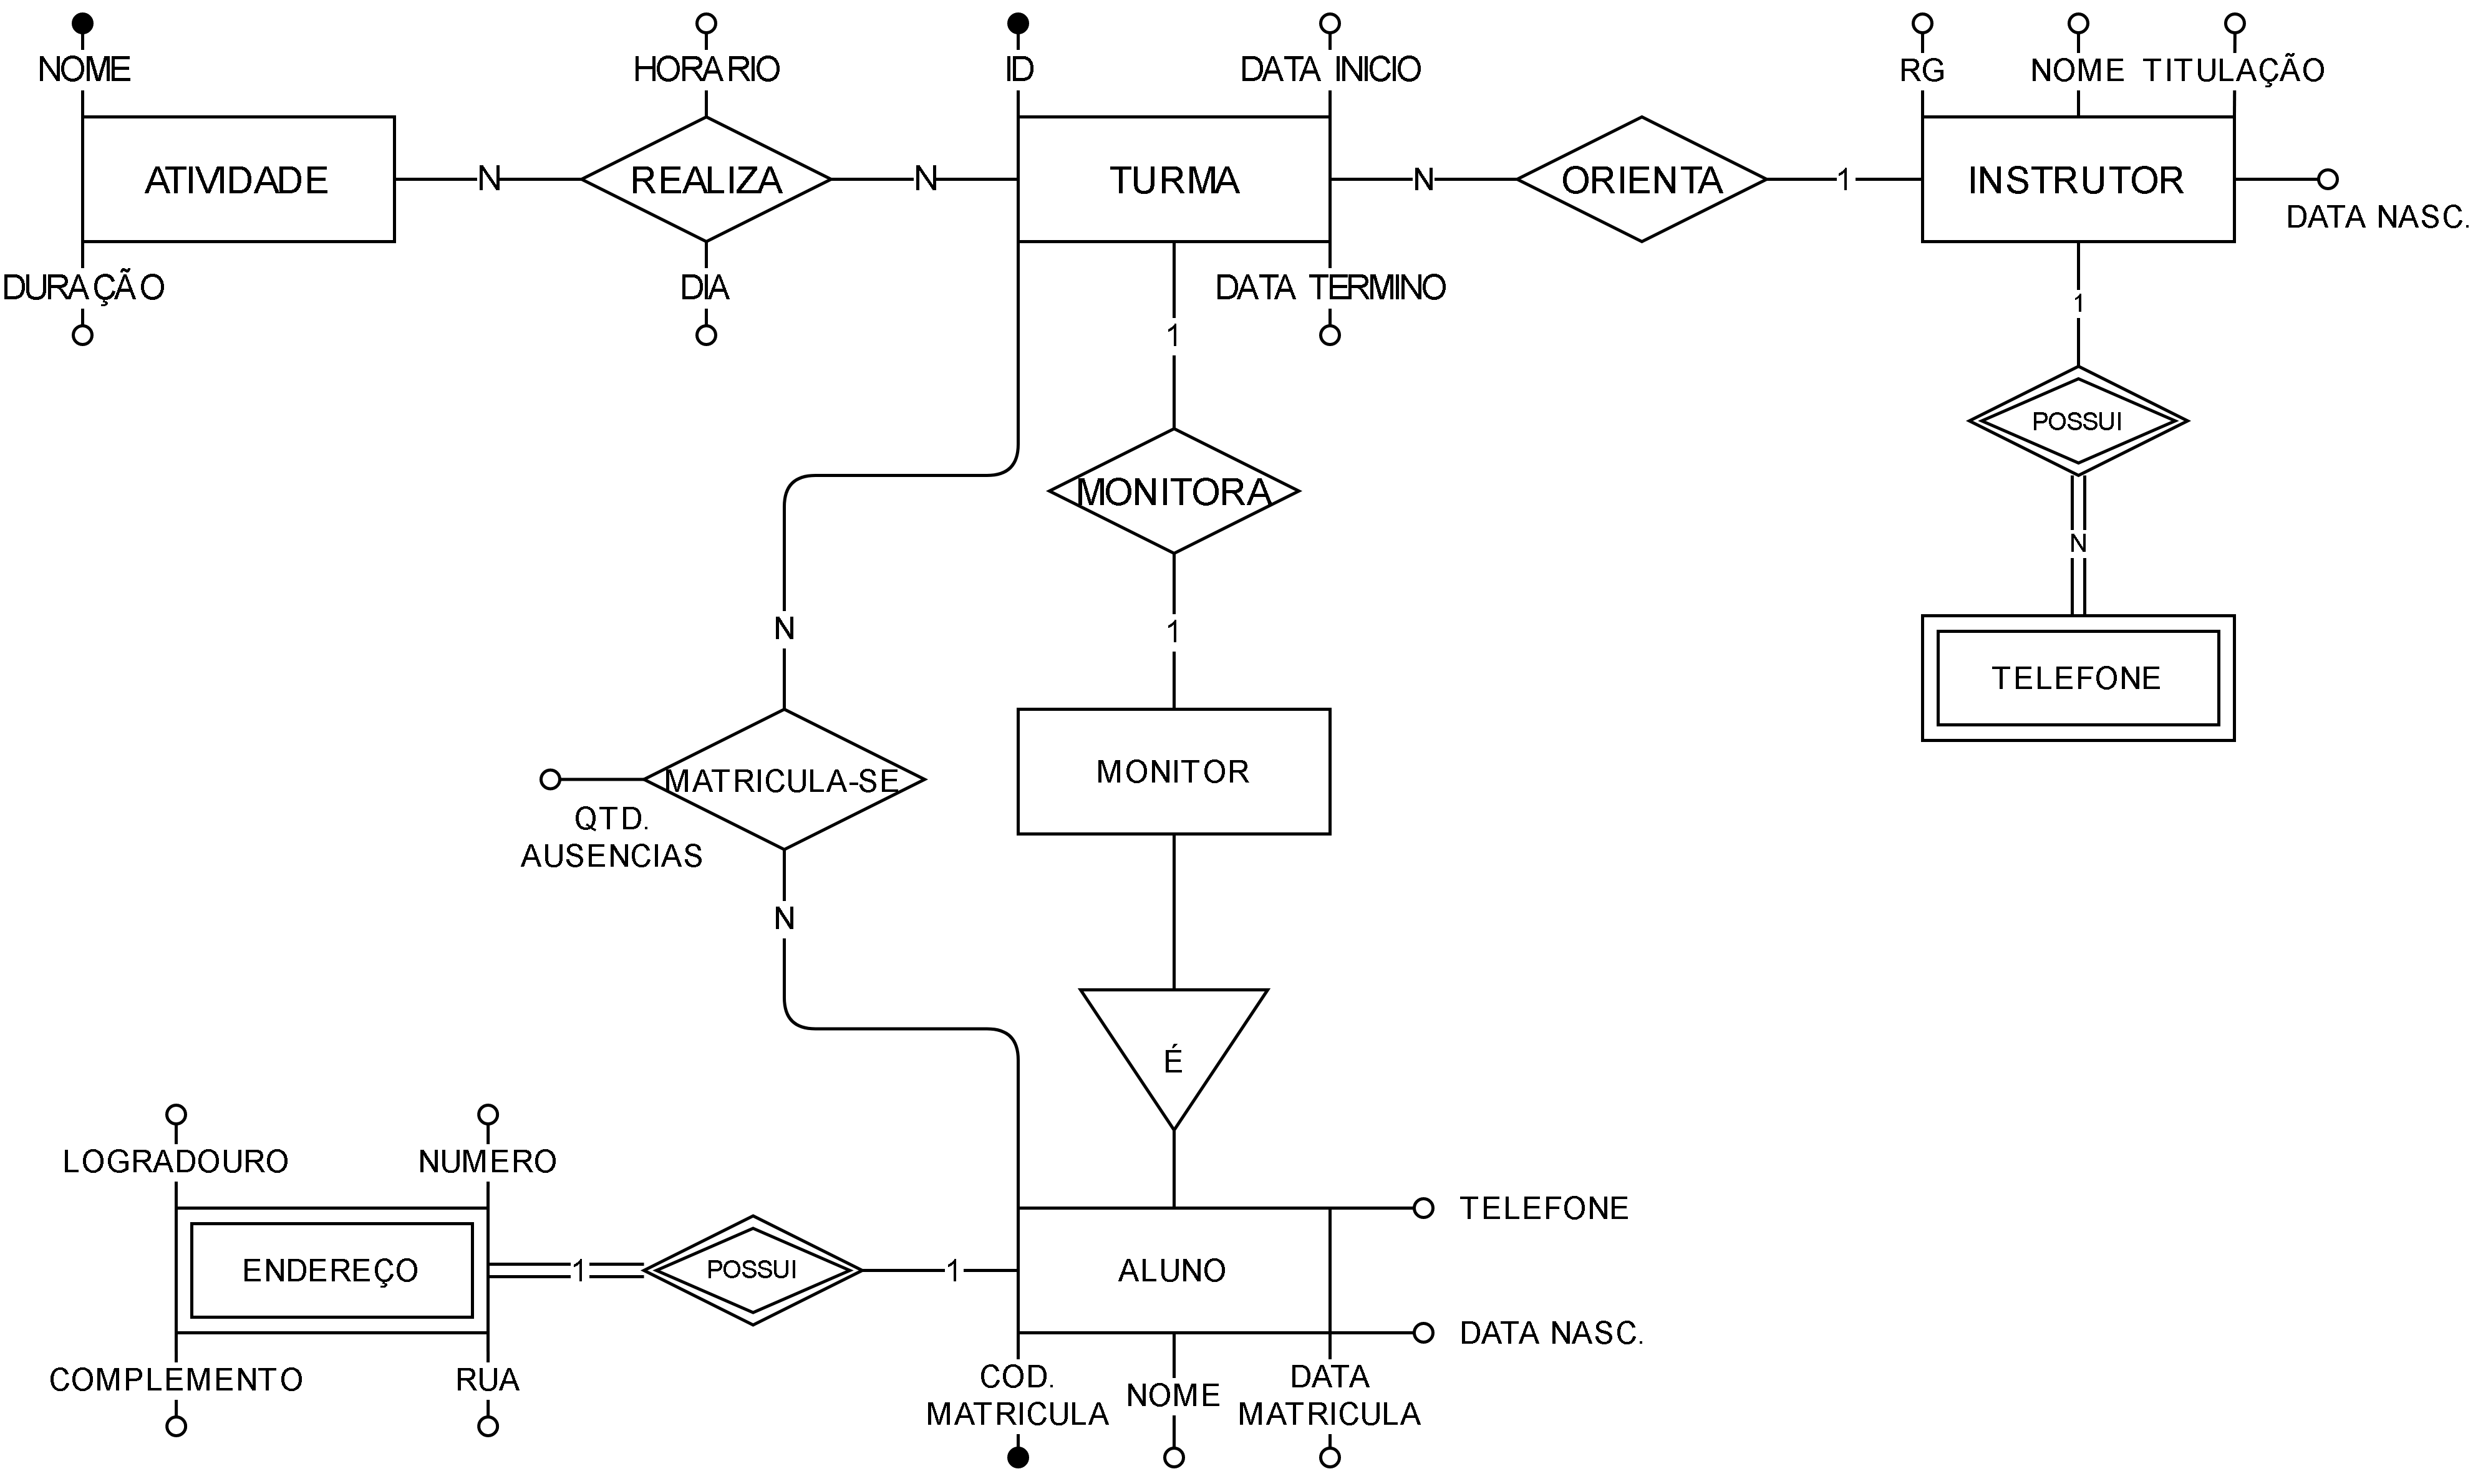
\includegraphics[width=1\textwidth]{ginastica.png}
		\end{figure}
	
		\newpage
		\item \textbf{[Aeroporto 1]}O aeroporto da Maringá resolveu organizar a sua informação num sistema de bases de dados. Para tal começaram por organizar a informação sobre os aviões "frequentam" o aeroporto.
		
		Cada avião tem um número de registo, e cada avião é de um modelo específico.
		O aeroporto pode acolher um certo número de modelos de aviões, e cada modelo tem um código de modelo (ex. DC-10, A320), bem como uma capacidade e um peso.
		Para todos os funcionários, é necessário guardar o seu nro. de BI, endereço, nro. de telefone e salário.
		Há funcionários que são técnicos. Cada técnico é perito num ou mais modelos de aviões, e vários técnicos podem ser peritos em modelos iguais.
		Há também funcionários controladores aéreos. Os controladores necessitam de ser sujeitos a um exame médico anual. Para cada controlador é necessário guardar a data do seu exame mais recente.
		Todos os empregados do aeroporto (técnicos e controladores) pertencem a um sindicato. É necessário guardar também o nro. de membro para cada empregado.
		O aeroporto tem um certo número de testes que são usados periodicamente para verificar o estado dos aviões. Cada teste tem um número atribuído pela Associação Nacional de Aeroportos (ANA), bem como um nome e uma pontuação máxima.
		
		\begin{figure}[H]
			\centering
			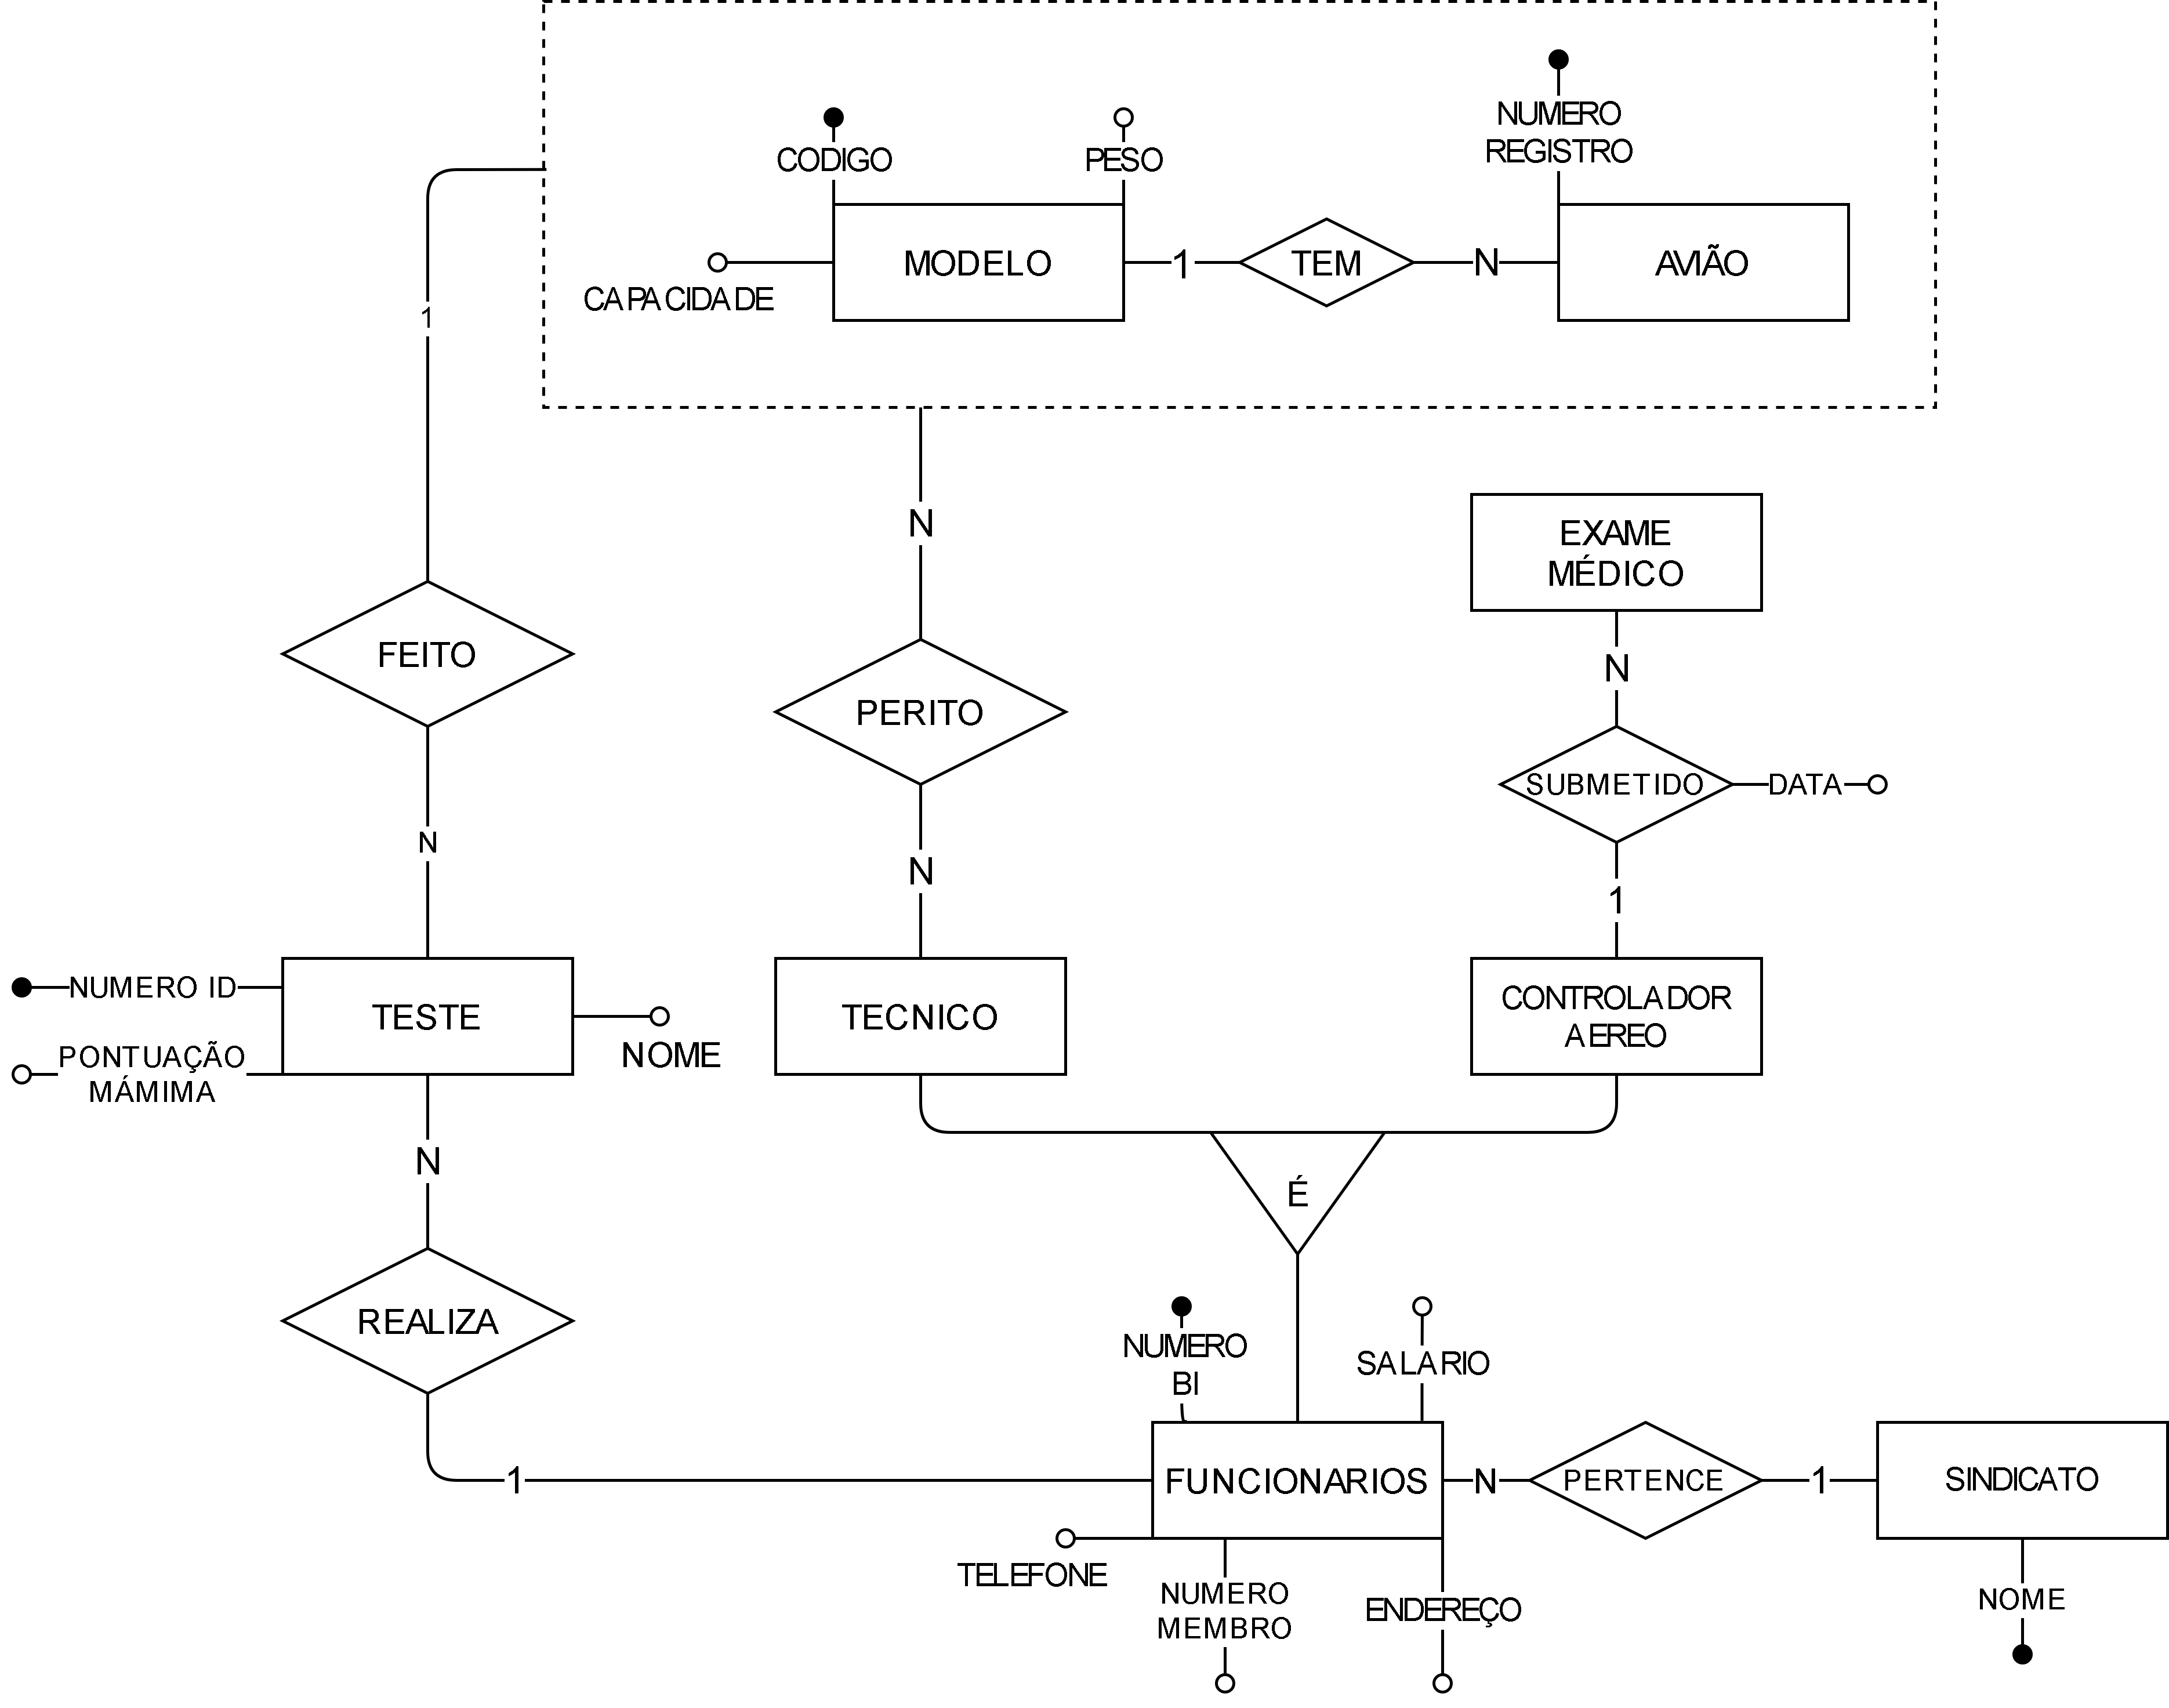
\includegraphics[width=0.9\textwidth]{aeroporto1.png}
		\end{figure}
	
		\newpage
		\item \textbf{[Aeroporto 2]}O aeroporto da Maringá resolveu organizar a sua informação num sistema de bases de dados. Para tal começaram por organizar a informação sobre os aviões "frequentam" o aeroporto.
		
		Cada avião tem um número de registo, e cada avião é de um modelo específico.
		O aeroporto pode acolher um certo número de modelos de aviões, e cada modelo tem um código de modelo (ex. DC-10, A320), bem como uma capacidade e um peso.
		Há técnicos em aeronaves que deve-se guardar o seu nro. de BI, endereço, nro. de telefone e salário.. Cada técnico é perito num ou mais modelos de aviões, e vários técnicos podem ser peritos em modelos iguais.
		O aeroporto tem um certo número de testes que são usados periodicamente para verificar o estado dos aviões. Cada teste tem um número atribuído pela Associação Nacional de Aeroportos (ANA), bem como um nome e uma pontuação máxima.
		A ANAC exige que o aeroporto mantenha informação sobre cada vez que um avião é sujeito a um determinado teste por um determinado técnico. Para cada teste efetuado, deseja-se guardar a sua data, o número de horas gastas pelo técnico, e a pontuação obtida pelo avião.
		
		\begin{figure}[H]
			\centering
			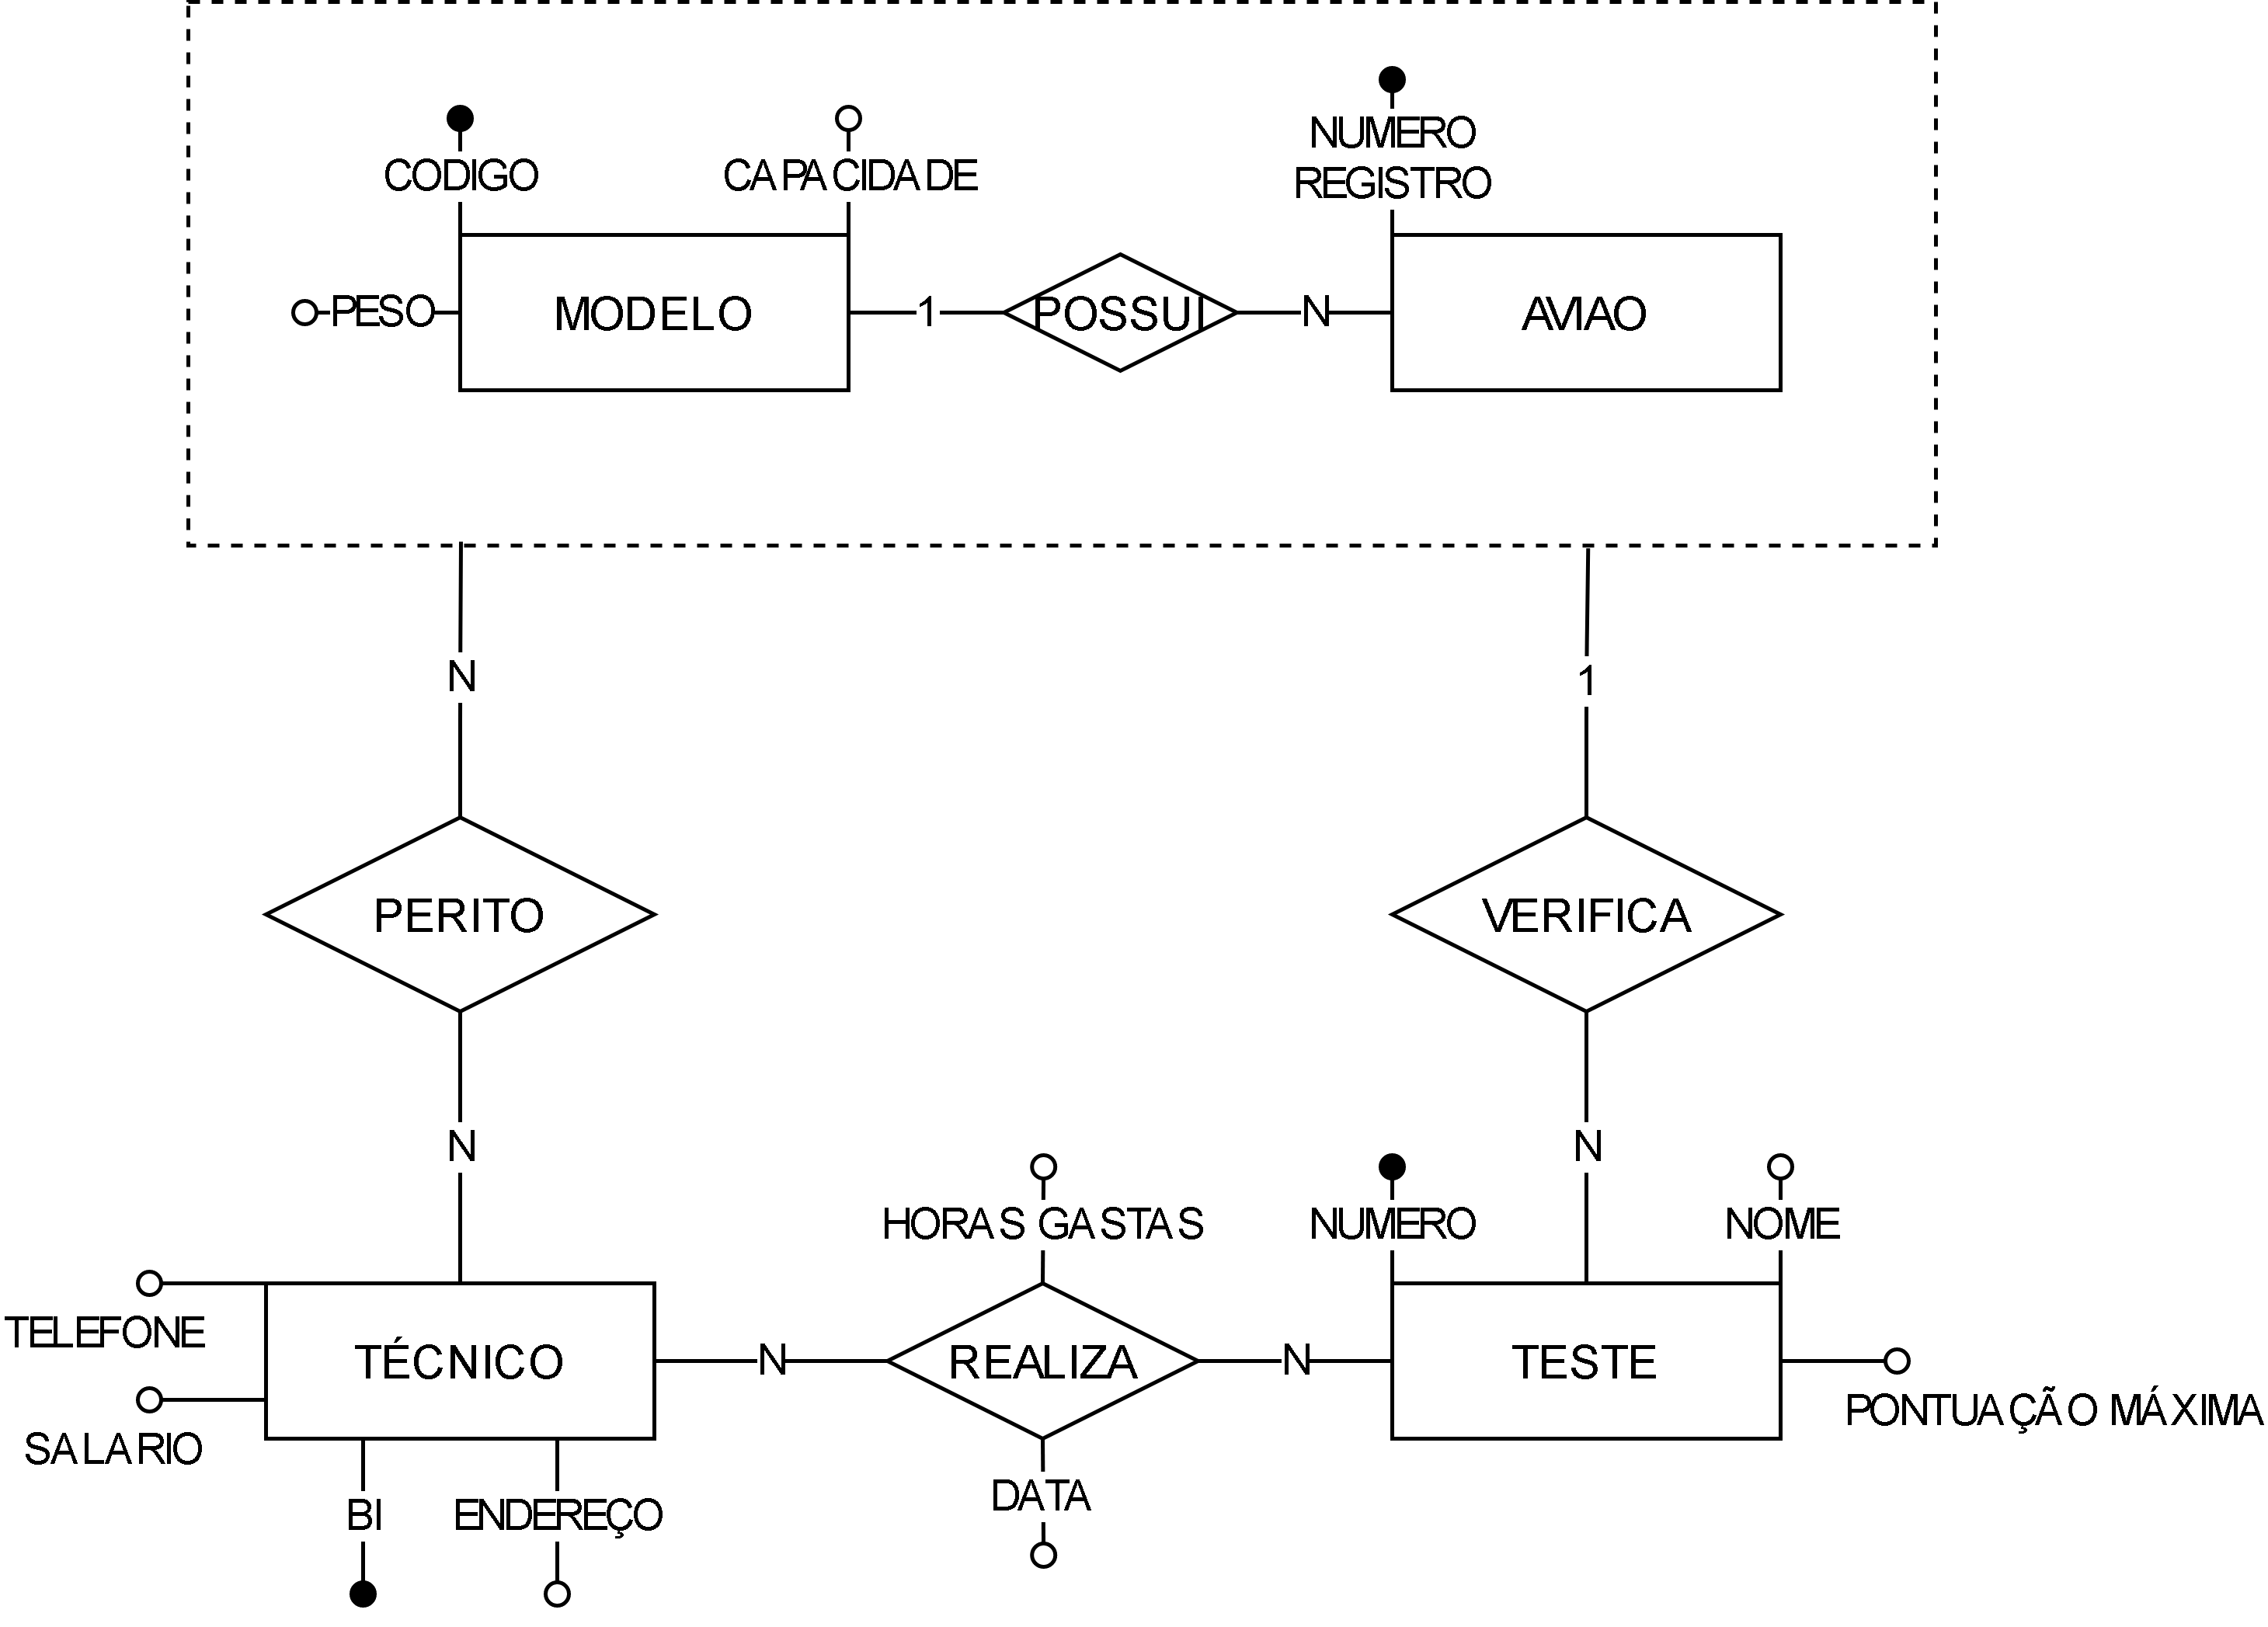
\includegraphics[width=1\textwidth]{aeroporto2.png}
		\end{figure}
		\newpage
		
		
		\item \textbf{[Farmácia] }A farmácia Prescrições-RX ofereceu a você um suprimento gratuito vitalício de medicamentos se você projetar seu banco de dados. Dados os custos crescentes relacionados aos cuidados com a saúde, você concordou. Eis as informações que você reuniu após a entrevista com seu cliente: 
		Os pacientes são identificados pelo CPF, e seus nomes, endereços e idades devem ser registrados.
		Os médicos são identificados pelo CPF. Para cada médico, o nome, especialidade e anos de experiência devem ser registrados.
		Cada empresa farmacêutica é identificada pelo nome e tem um número de telefone.
		Para cada remédio, o nome e a fórmula devem ser registrados. Cada medicamento é vendido por determinada empresa farmacêutica, e o seu nome o identifica univocamente entre os produtos dessa empresa. Se uma empresa farmacêutica é excluída, você não precisa mais manter o controle de seus produtos.
		Todo paciente tem um médico principal. Todo médico tem no mínimo um paciente.
		A farmácia vende diversos medicamentos e mantém um preço para cada um.
		Os médicos prescrevem medicamentos para os pacientes. Um médico pode prescrever um ou mais medicamentos a diversos pacientes e um paciente pode obter prescrições de diversos médicos. Cada prescrição tem uma data e uma quantidade associada a ela. Você pode assumir que, se um médico prescreve o mesmo medicamento para o mesmo paciente mais do que uma vez, apenas a última prescrição precisa ser armazenada.
		
		\begin{figure}[H]
			\centering
			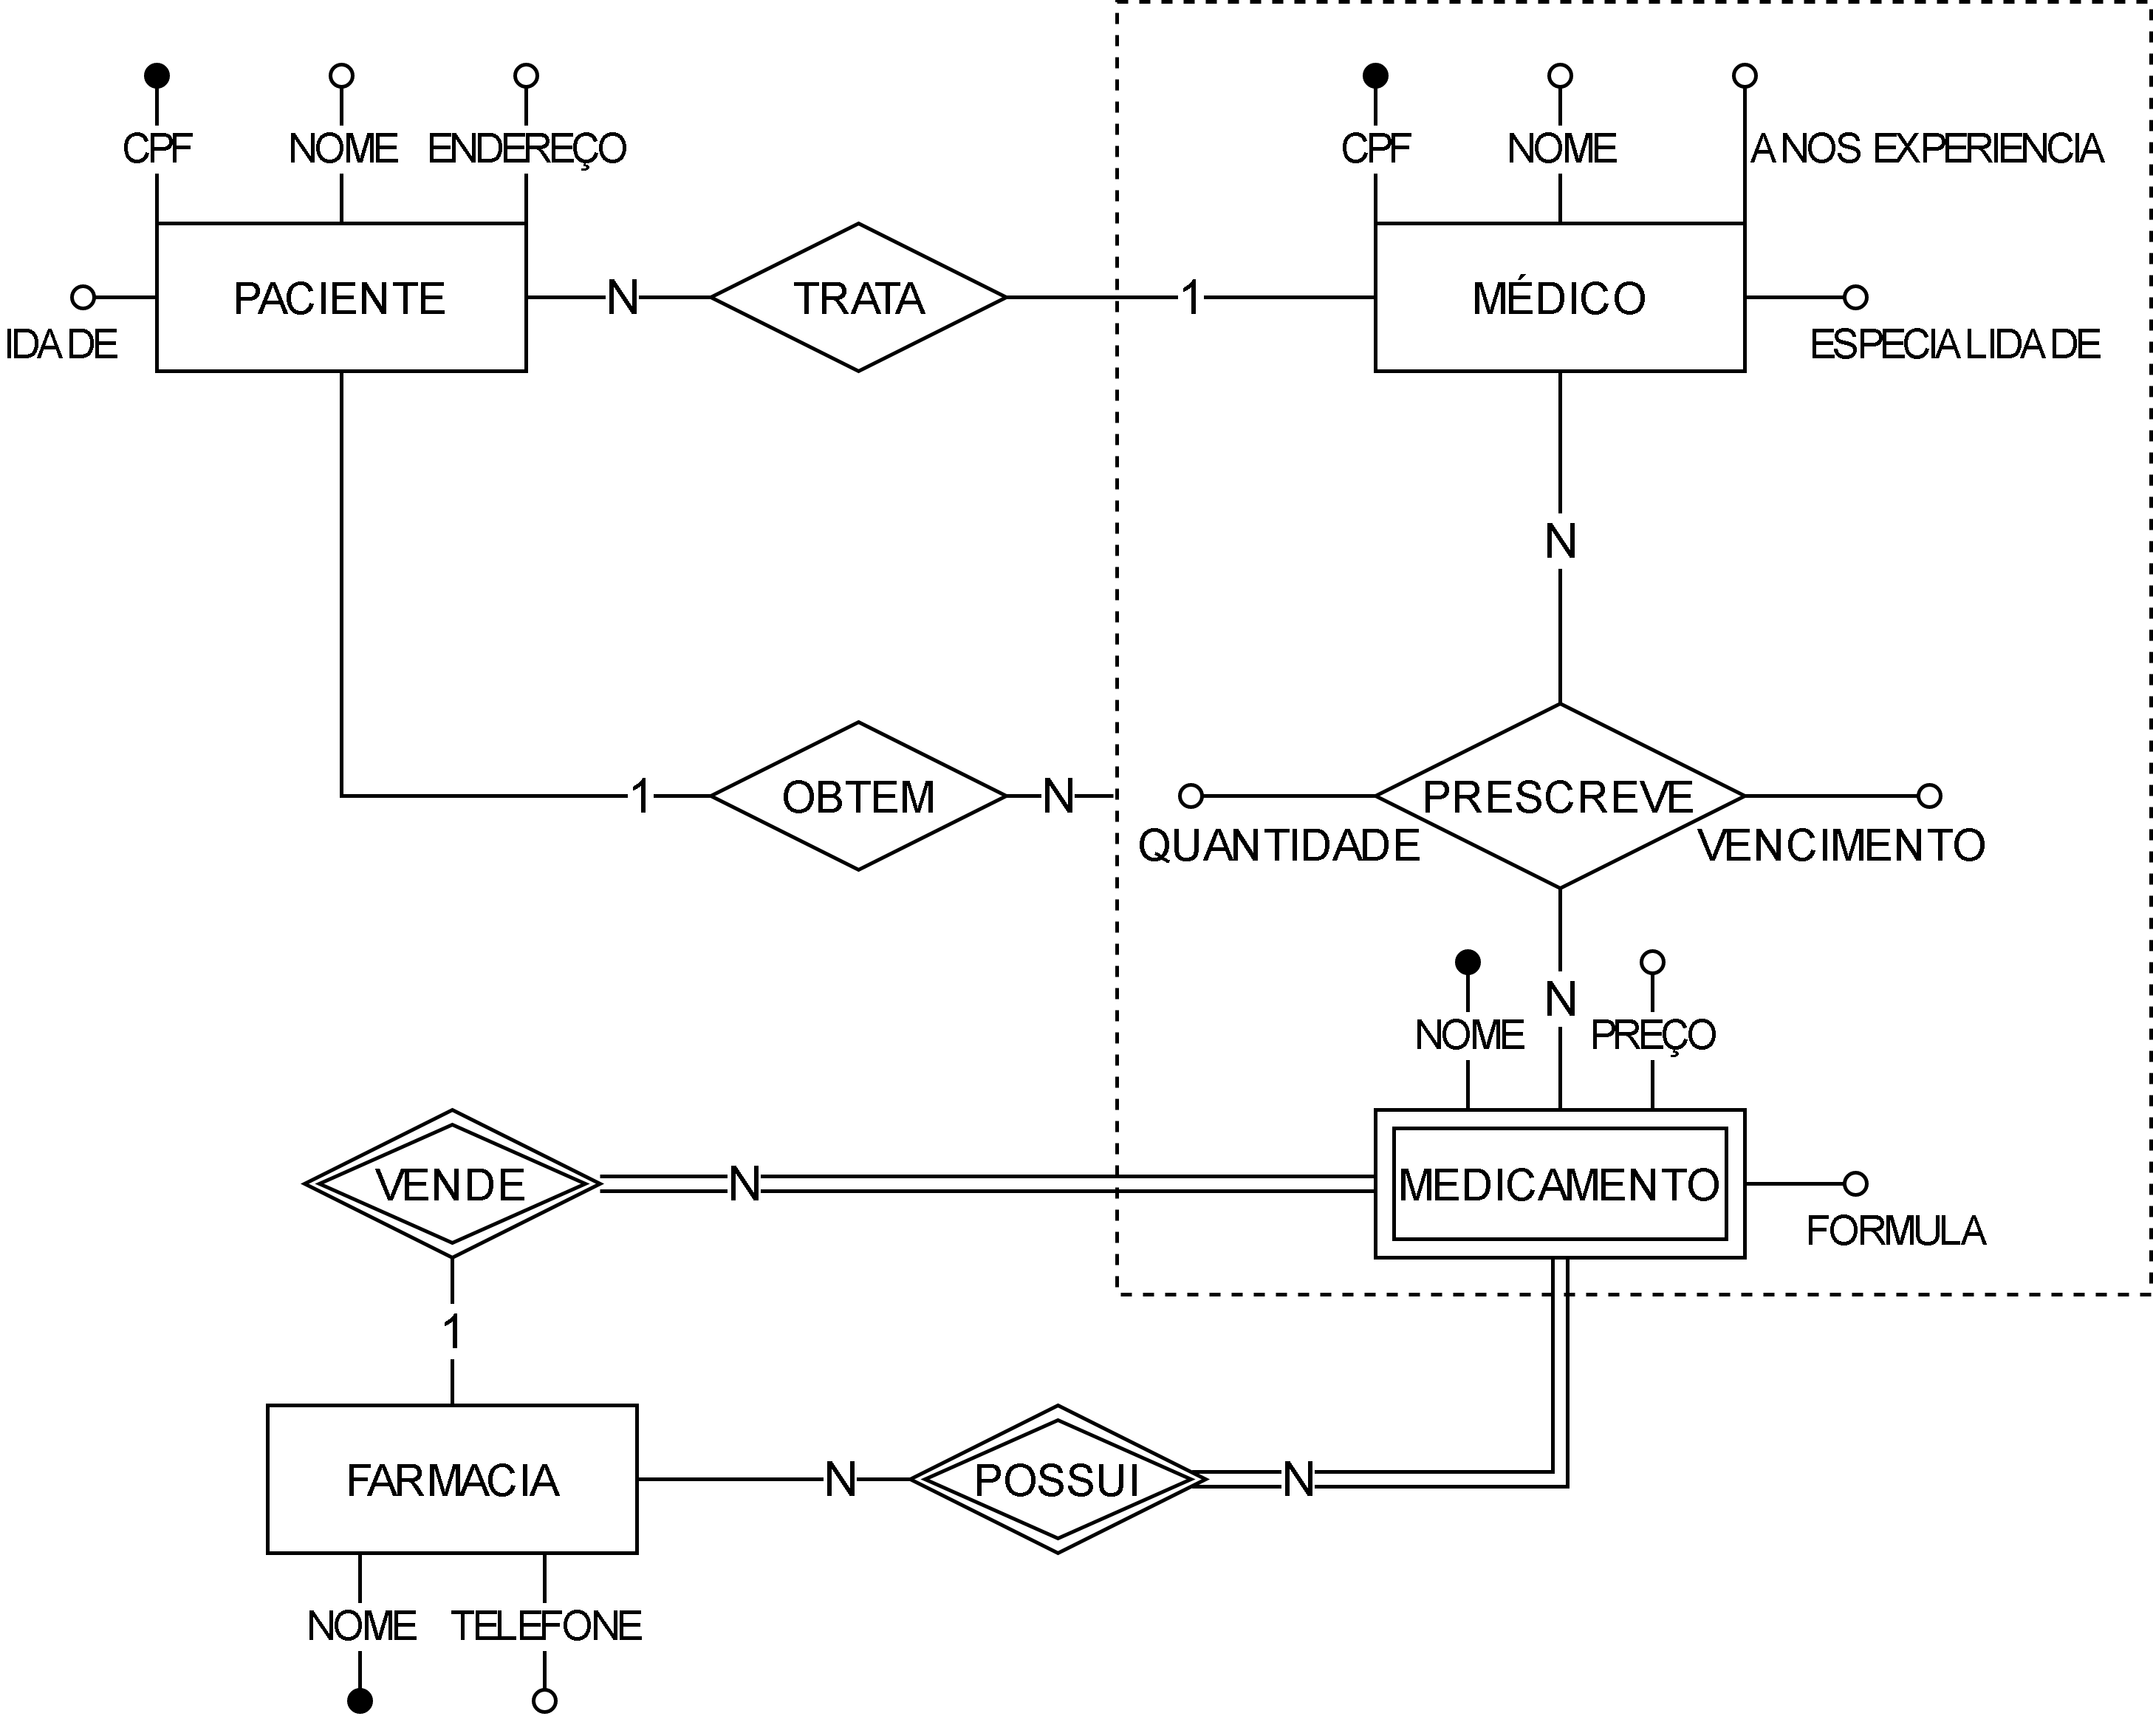
\includegraphics[width=0.82\textwidth]{farmacia.png}
		\end{figure}
		\newpage
		
		\item \textbf{[Agência de Emprego]} Uma empresa de agenciamento de mão de obra pretende informatizar o cadastro de profissionais candidatos a empregos temporários. Pretende-se construir um banco de dados onde possa manter os dados cadastrais dos profissionais e seus contratos temporários com os contratantes. O profissional é identificado por um número de controle e além desta identificação ficam registrados seu nome, endereço, nascimento e profissão. Os contratos de mão de obra temporária são feitos individualmente (um contrato para cada profissional) com os contratantes. Cada contrato é identificado por um número único e nele são registrados a vigência do contrato (data de início e de término) e o valor pago por hora trabalhada. Um contratante, quando pessoa jurídica, possuem CNPJ, razão social, nome e endereço. Já quando o contratante é uma pessoa física, ele possuem CPF, nome e endereço.
		
		
		\begin{figure}[H]
			\centering
			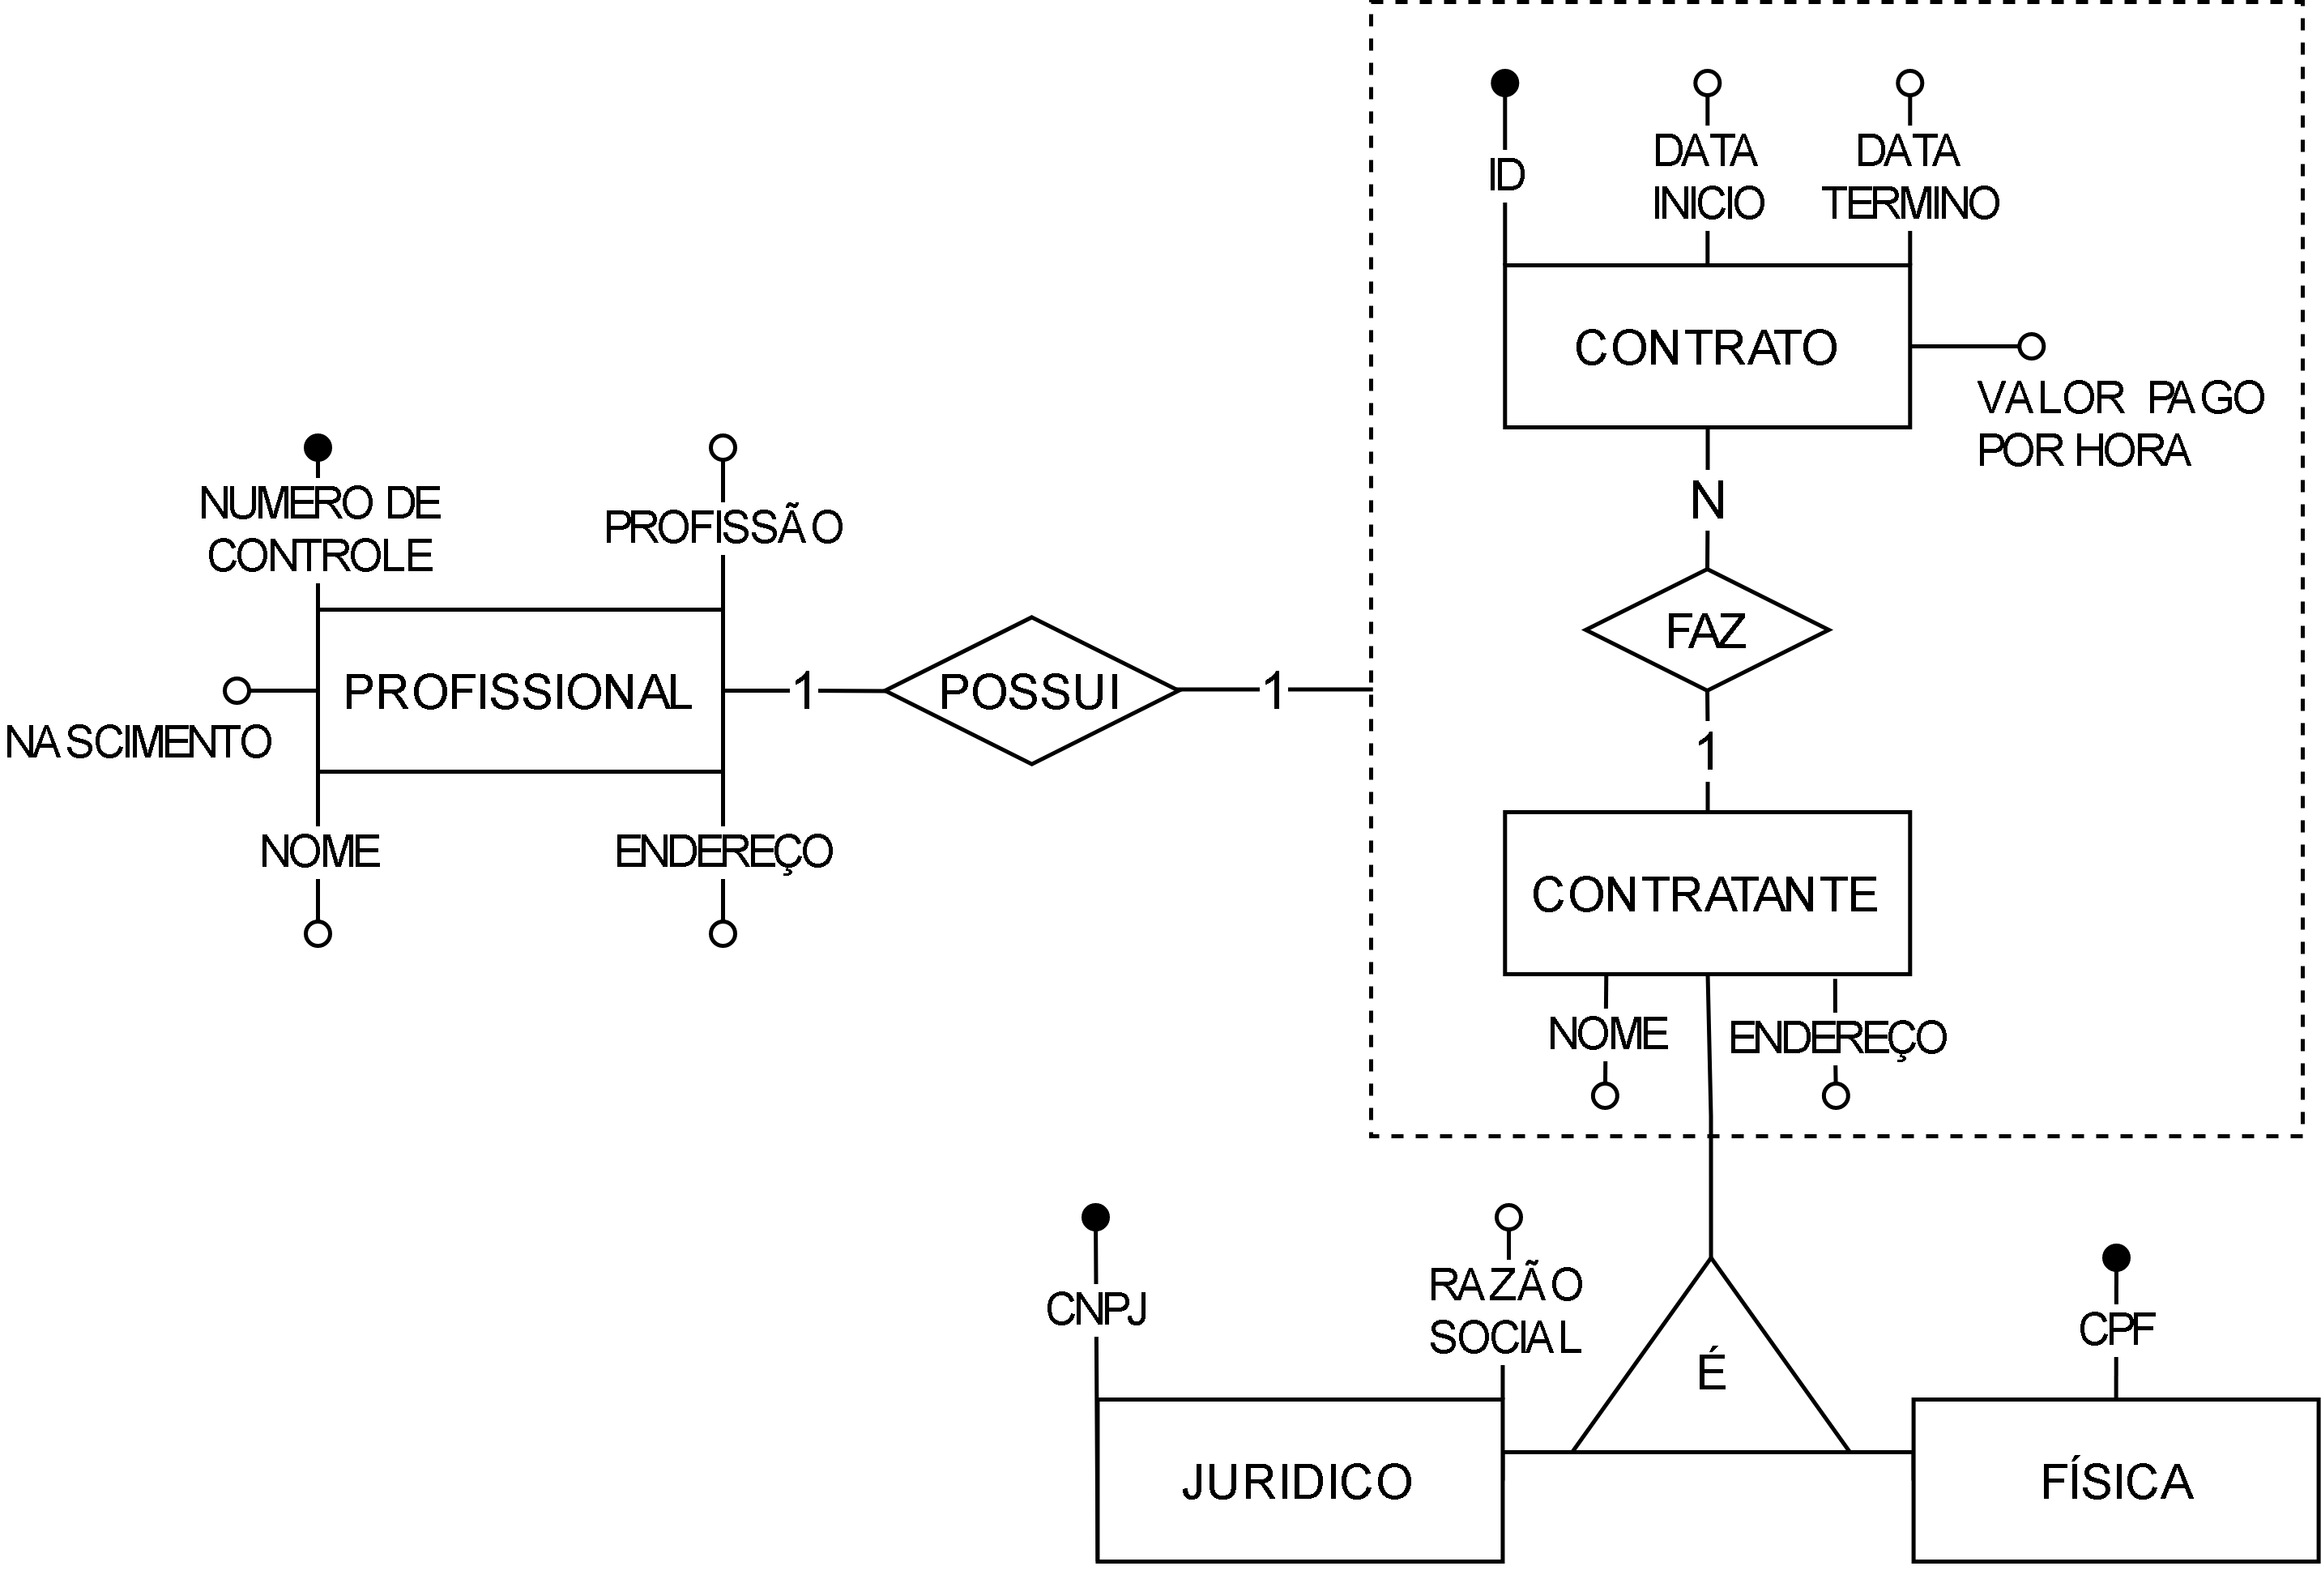
\includegraphics[width=1\textwidth]{agenciaEmprego.png}
		\end{figure}
		\newpage
		
		\item \textbf{[Copa do Mundo de Futebol]} Construa um modelo de entidade-relacionamento \textbf{(MER)} para uma empresa jornalística que deseja construir uma base de dados para armazenar resultados passados de copas do mundo de futebol, para acesso por seus repórteres. A base de dados armazena informações sobre países que participaram ou sediaram copas do mundo. Cada país é identificado por uma sigla de duas letras e possui um nome. Uma copa é identificada pelo ano em que ocorreu e a base de dados armazena as datas de início e fim da copa, bem como o nome da cidade em que ocorreu a cerimônia de abertura. Para cada copa, cada país monta uma equipe diferente de jogadores. Cada equipe tem um treinador e vários jogadores. Tanto treinadores, quanto jogadores estão armazenados em uma base de dados de pessoas, cada uma identificada por um código. Para as pessoas, a base de dados mantém, além do código, seu nome, data de nascimento, e país de nascimento. Observar que uma pessoa pode participar de diferentes copas e com diferentes papéis (treinar e jogador). Finalmente, deseja-se armazenar os jogos ocorridos em cada copa. Os jogos são numerados de um em diante dentro de cada copa. Para cada jogo deve-e saber o nome do estádio em que ocorreu, a data e hora do jogo, as equipes que dele participaram, bem como o número de gols em cada equipe.
		
		\begin{figure}[H]
			\centering
			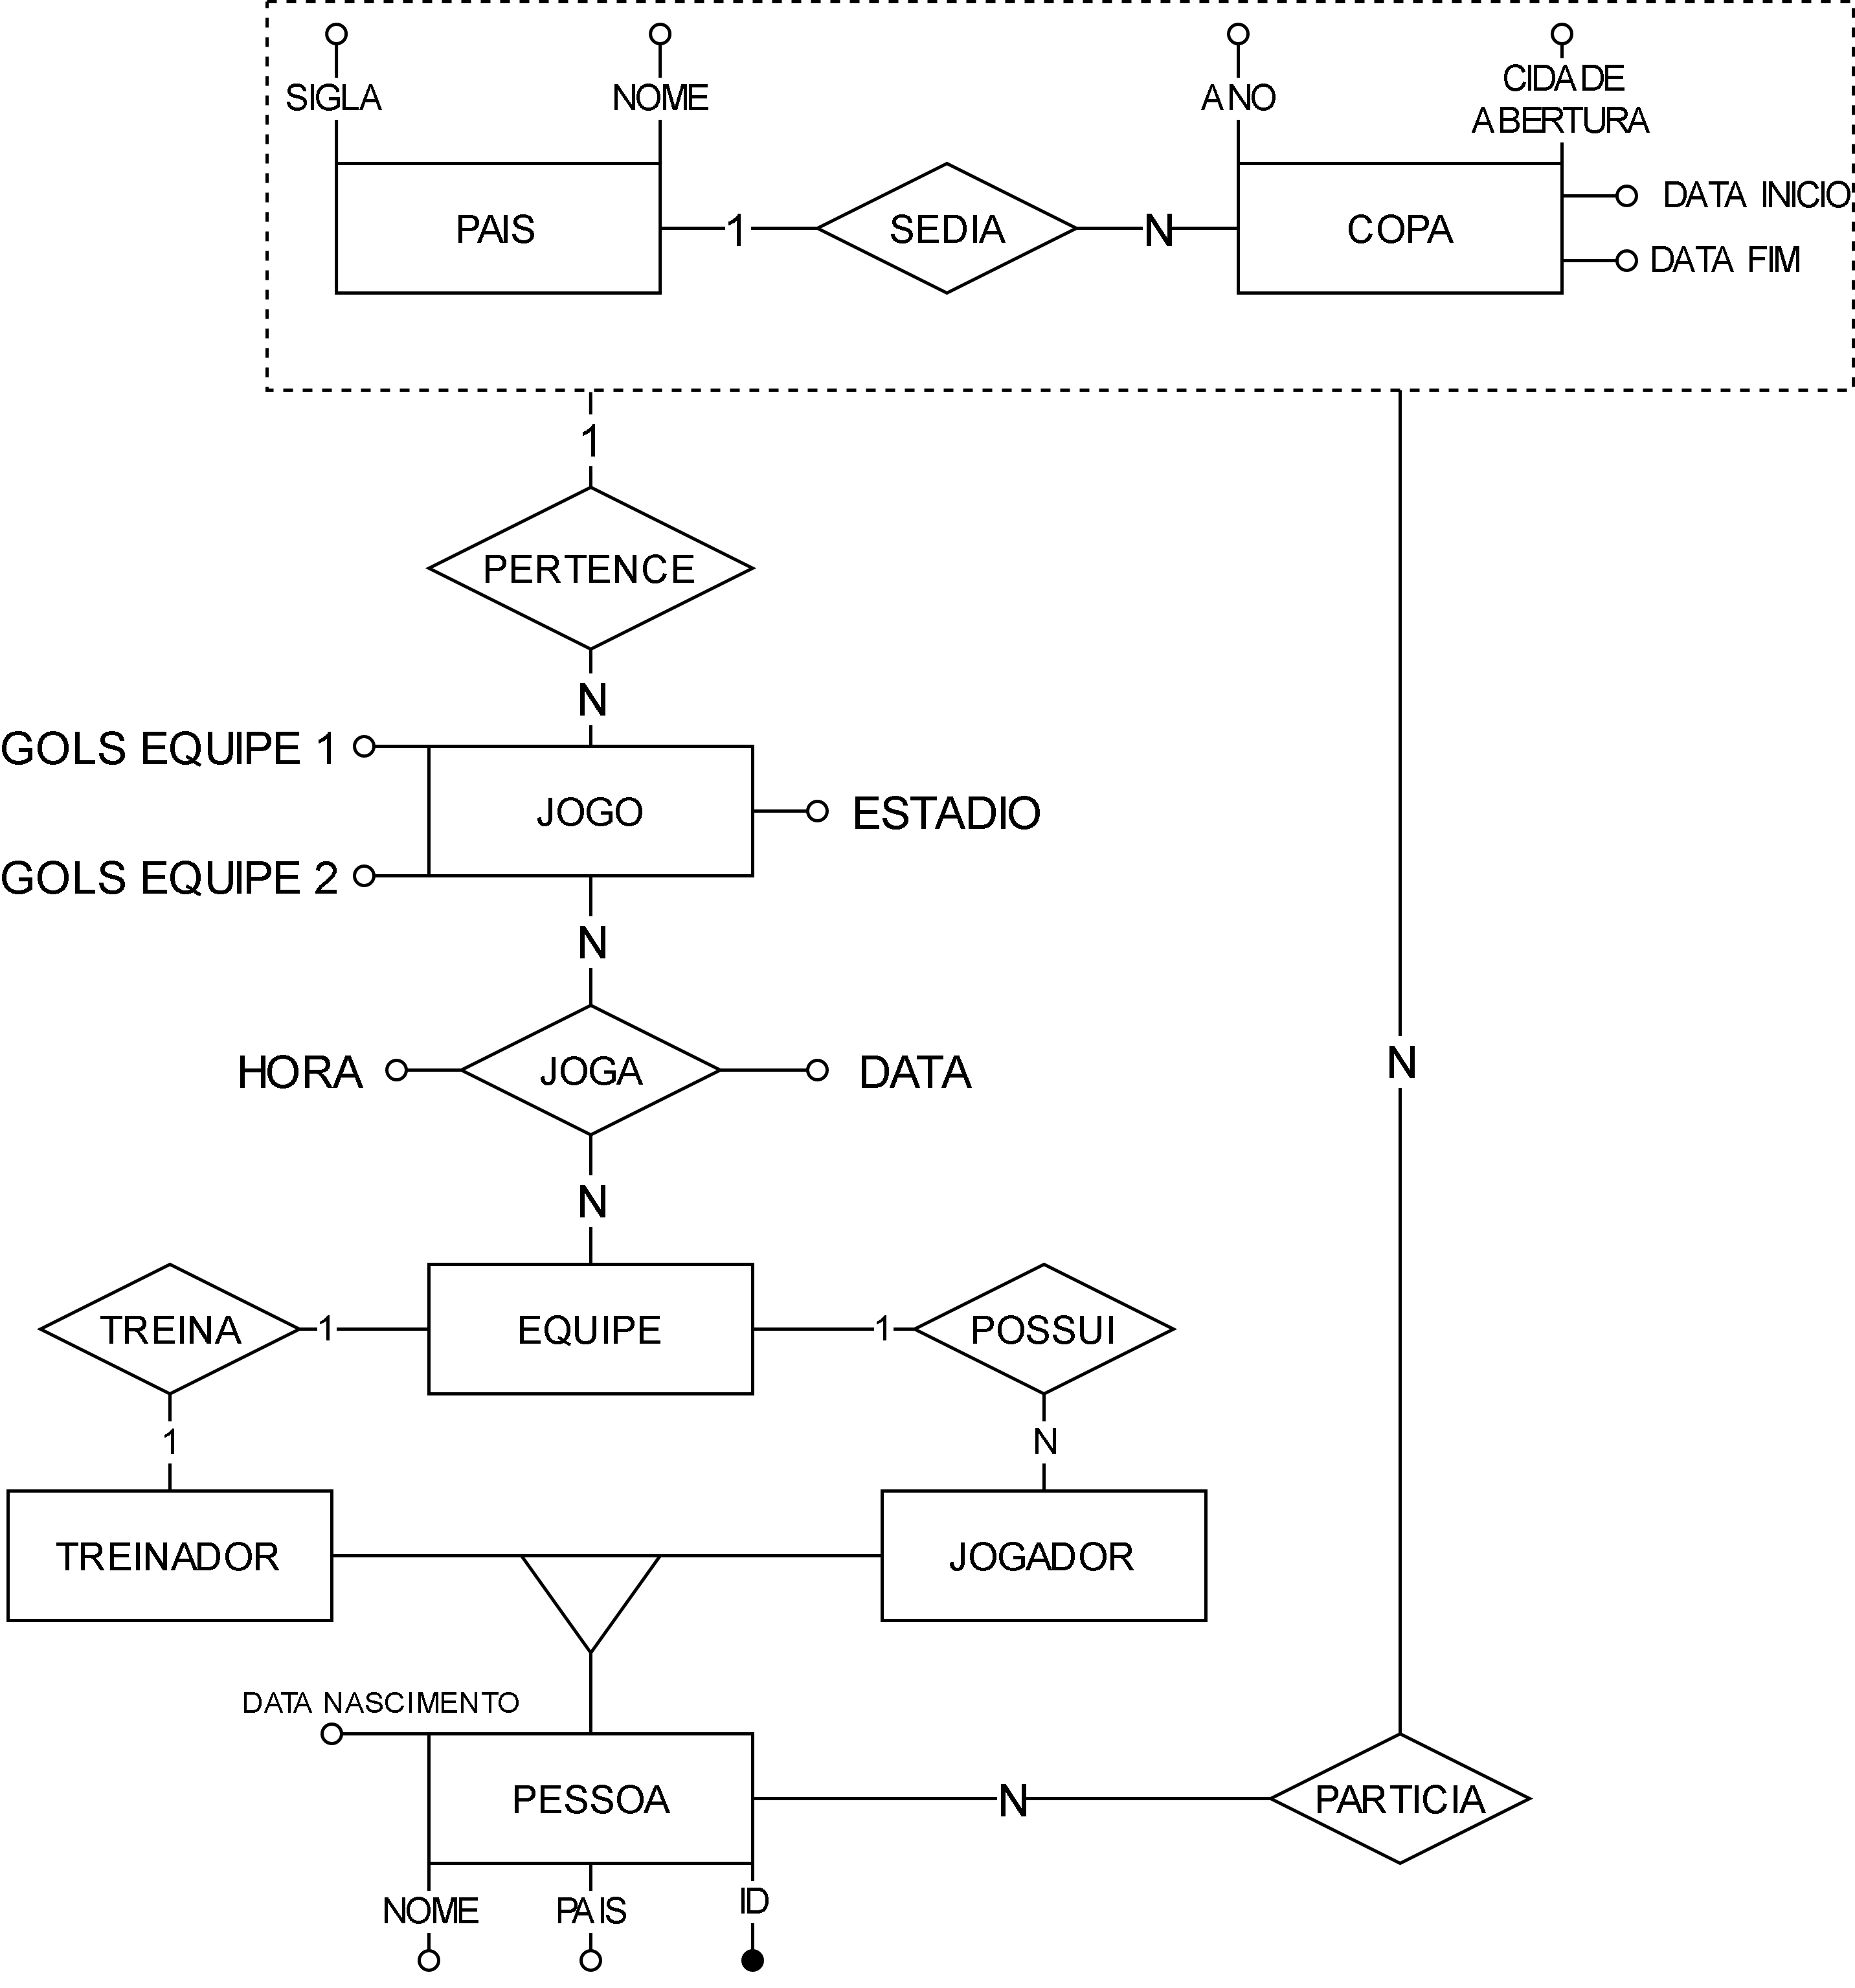
\includegraphics[width=0.65\textwidth]{copaDoMundo.png}
		\end{figure}
		\newpage
		
	\end{enumerate}
		
\end{document}
